\documentclass[12pt,journal]{IEEEtran}
\usepackage[
  backend=biber,
  style=numeric,
  citestyle=numeric
]{biblatex}
\usepackage{graphicx}
\addbibresource{citations.bib}
\providecommand{\keywords}[1]{\textbf{Keywords} #1}
\begin{document}
\title{Traffic Analysis on Tor}
\author{\IEEEauthorblockN{William Liddy\IEEEauthorrefmark{1}, Brian Pollack\IEEEauthorrefmark{2}}\\
        \IEEEauthorblockA{Department of Electrical Engineering and Computer Science\\Case Western Reserve University\\Cleveland, OH 44106\\\IEEEauthorrefmark{1}wjl36@case.edu, \IEEEauthorrefmark{2}bmp55@case.edu}}
\maketitle

\begin{abstract}
TODO: Abstract
\end{abstract}

% \keywords\\{TOR; Onion Routing, }

\section{Introduction}
\IEEEPARstart{T}{his} is the introduction.

\section{Background}
\subsection{Tor Architecture}
Tor is a circuit-based anonymous communication service that uses Onion Routing to securely pass packets in the network. Onion Routing is an overlay network protocol that is designed to carry TCP packets over existing networks. Traffic flows through the network in fixed size segments. Each node unwraps a layer from the packet using a symmetric key and forwards it to the next node. The packet is unwrapped like an union, which is where the name comes from.
\par
Tor routes its traffic using circuits. A user will set up a circuit using at least three Tor nodes, and that circuit stays active until the user either is finished or requests a new circuit. Tor circuits can carry most TCP applications (HTTP, SSH, etc.), however cannot carry UDP packets. A single Tor circuit can carry multiple simultaneous streams, which is good for HTTP traffic which opens multiple connections to multiple destinations.
\par
While some anonymity services will reorder, mix, or otherwise shape the traffic flowing between Onion Routers, Tor chooses to not attempt to shape the traffic. The creators believed that all currently available traffic shaping strategies were still vulnerable to attacks and were difficult to implement practically. They also wanted to make Tor as low-latency as possible, and reordering packets would increase latency. Tor simply sends traffic in a round robin fashion.
\par
To protect against traffic bottlenecks, Tor uses a decentralized congestion control mechanism that sends end-to-end ack packets to maintain anonymity while allowing edge nodes to detect congestion and throttle their traffic until congestion subsides.
\par
Traffic is only allowed to leave the Tor network through nodes which specifically allow exits (called exit nodes). Each node has a policy stating which traffic is allowed to leave the network: this can be restricted by IP address or protocol. \cite{Dingledine:2004:TSO:1251375.1251396}

\subsection{Tor Threat Model}
Tor is designed to be impossible for attackers to link users with the services to which they are connecting \cite{Dingledine:2004:TSO:1251375.1251396}. The main goal of most attackers to the Tor network, therefore, is to de-identify its users and observe the remote services they are accessing. The attacker would then be limited by other encryption protocols, such as HTTPS, but that is beyond the scope of our study. A secondary goal of an attacker would be to group network connections, establishing a link among multiple connections to the same initiator. This would allow the attacker to build a profile on the user be observing with whom the user is communicating and by observing the user’s communication habits \cite{Murdoch:2005:LTA:1058433.1059390}.
\par
Tor is designed to protect against an adversary who can observe some fraction of network traffic. This adversary can generate, modify, delete, or delay traffic and can operate his or her own tor nodes. The adversary can also compromise some fraction of existing tor nodes\cite{Dingledine:2004:TSO:1251375.1251396}.
\par
Additionally, it is important to note that Tor does not protect against traffic confirmation attacks, which are when an adversary suspects two parties are communicating and tries to prove it by analyzing the network. Tor rather attempts to make it difficult to identify who is communicating without a solid suspicion \cite{Murdoch:2005:LTA:1058433.1059390}.
\par
With our attacks, we try to gain information about the path of the Tor circuit using methods available to all Tor users. It is important to note that we do not exit the threat model for which Tor is built. We demonstrate that small attackers are able to gain insights about Tor users. This means that both government and non-government agencies are able to carry out these attacks on Tor.

\subsection{Previous Work}
In 2005, Murdoch and Danezis studied similar attacks to the Tor network. They assumed that an adversary created a corrupt Tor node on the network. The corrupt node is then used to measure other nodes' traffic load. Additionally, they assumed that the attackers controlled a network server that the user to be traced is accessing. Murdoch and Danezis claim that this threat is within the threat model that should be covered by Tor. If the attackers modulate the data through the network server that the user is accessing, they were able to observe similar modulations in the Tor circuit that the user was using. This means, therefore, that the attackers could trace the user through the Tor circuit and link a user with the services he or she is using \cite{Murdoch:2005:LTA:1058433.1059390}. Figure \ref{murdochsetup} shows Murdoch and Danezis's attack setup.
\begin{figure*}

 \center
  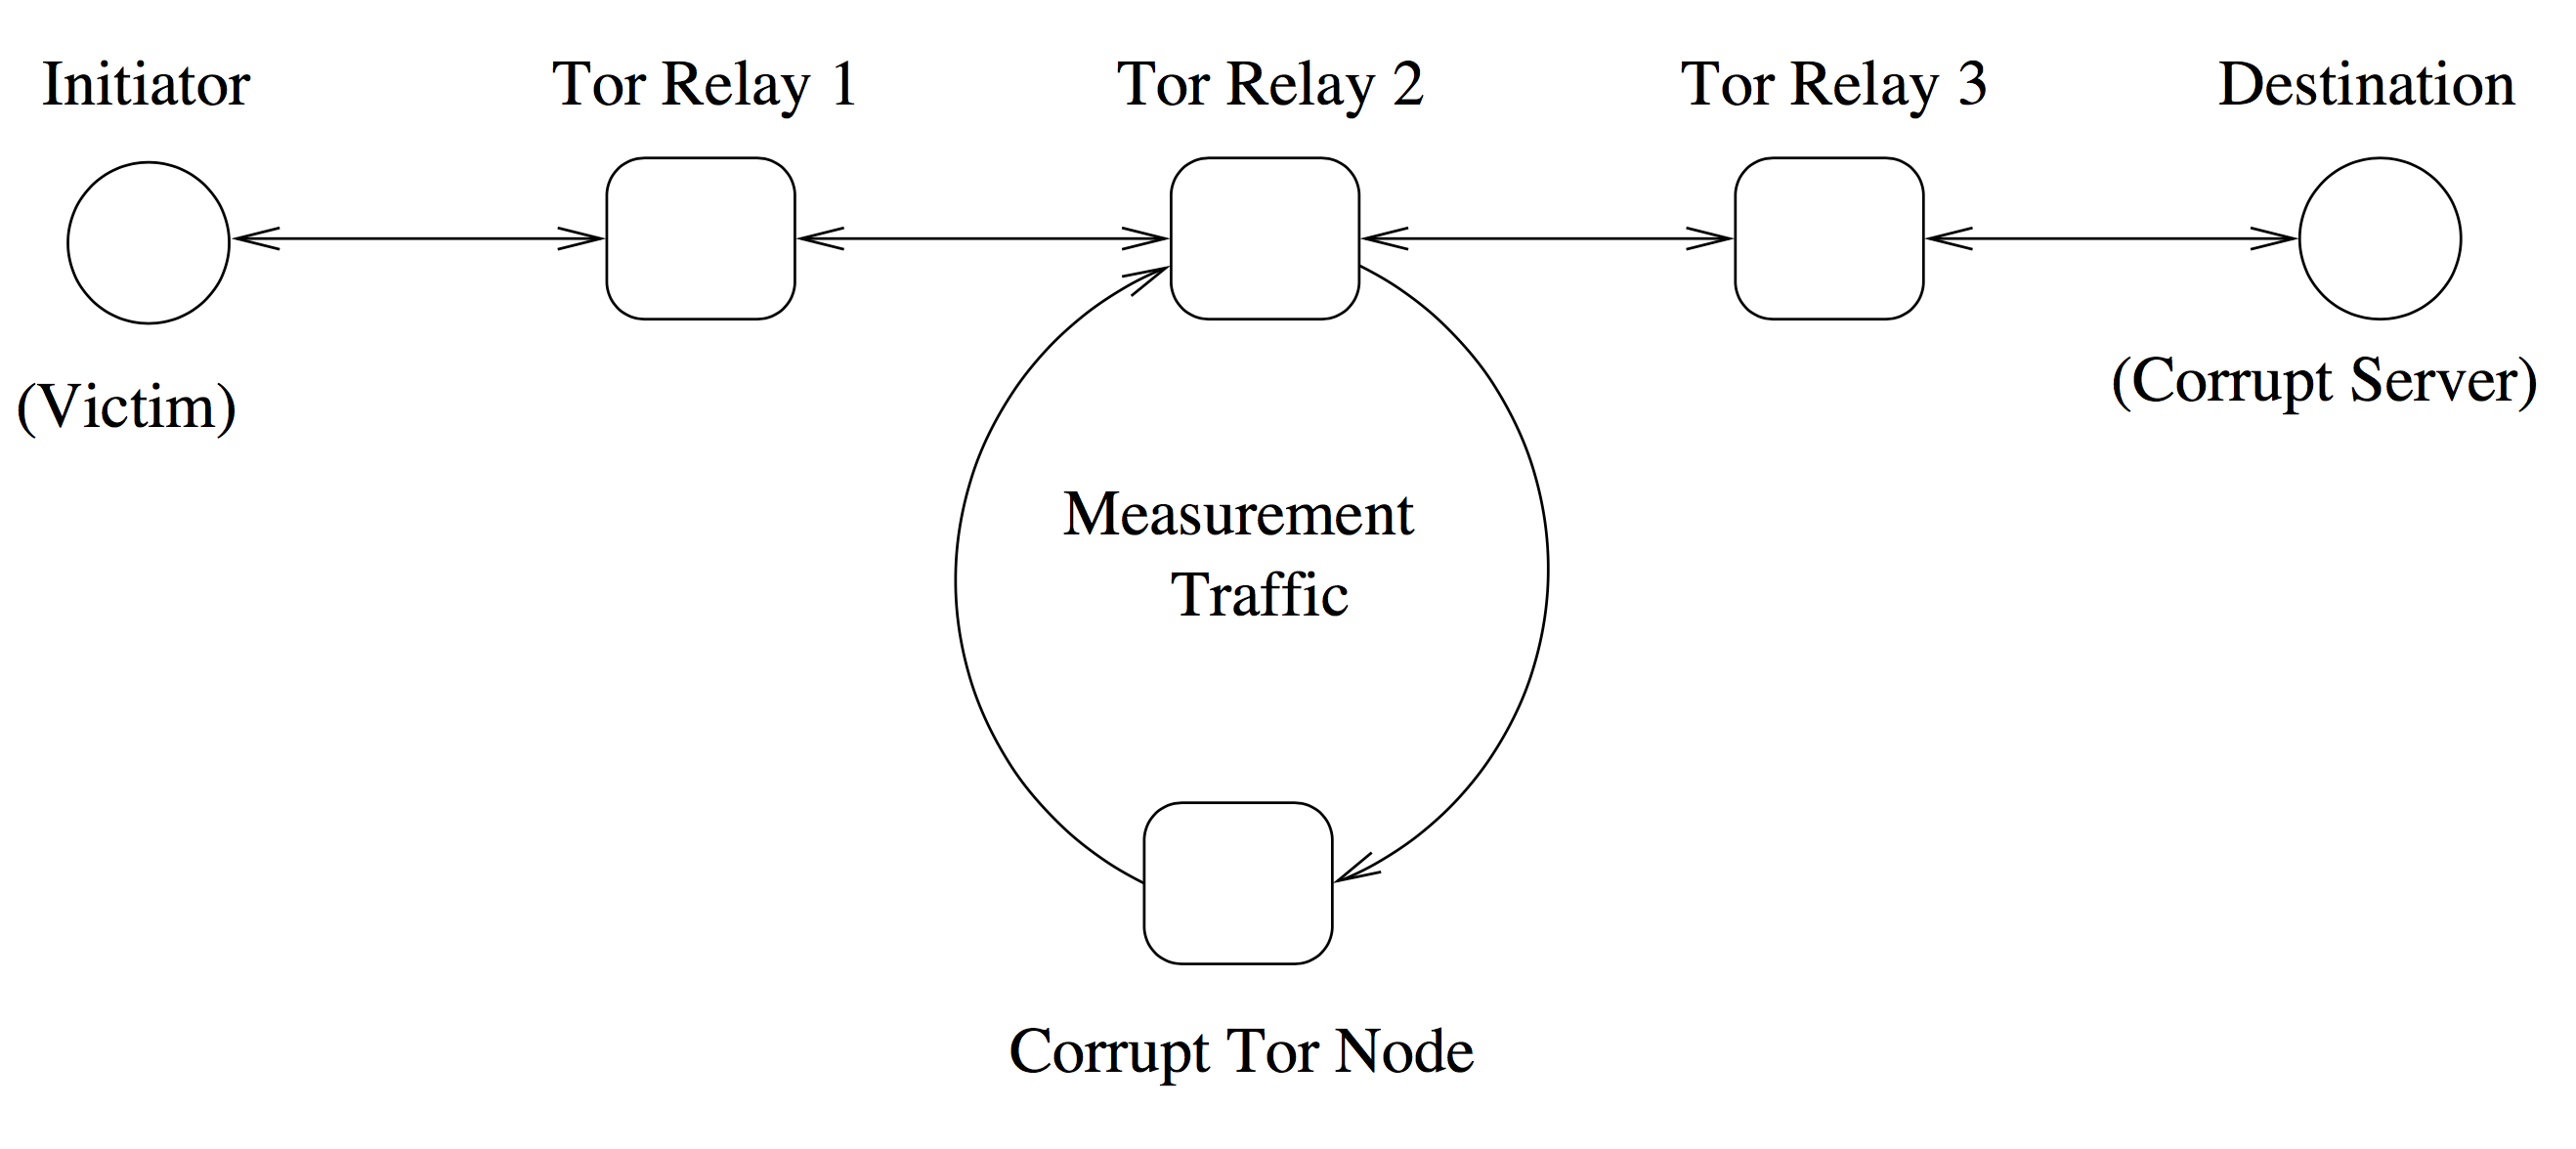
\includegraphics[width=\textwidth]{figures/murdochattacksetup.png}
  \caption{Murdoch and Danezis's Attack Setup}
  \label{murdochsetup}
\end{figure*}

\section{Our Setup and Results}
We wanted to test to see if the Tor network was still vulnerable to Murdoch and Danezis's attack. We did not simply duplicate their attack. Rather, we modified it slightly and reevaluated the exact attack scenarios. We wanted to demonstrate that this attack has significant real world implications that need to be addressed by the Tor network.
\subsection{Consensus Values}
When a Tor node is first created, it goes through four phases as it is being added to the Tor network. Each phase allows a different amount of traffic to be routed through the new node.
\subsubsection{Phase 1: unmeasured}
When a relay is first started, it will self-test its bandwidth. It publishes the results to its relay descriptor. For the first few days, the Tor network will allow only 20KB/s of bandwidth through the new node.
\subsubsection{Phase 2: remote measurement}

\printbibliography
\end{document}
